\documentclass[english,man]{apa6}

\usepackage{amssymb,amsmath}
\usepackage{ifxetex,ifluatex}
\usepackage{fixltx2e} % provides \textsubscript
\ifnum 0\ifxetex 1\fi\ifluatex 1\fi=0 % if pdftex
  \usepackage[T1]{fontenc}
  \usepackage[utf8]{inputenc}
\else % if luatex or xelatex
  \ifxetex
    \usepackage{mathspec}
    \usepackage{xltxtra,xunicode}
  \else
    \usepackage{fontspec}
  \fi
  \defaultfontfeatures{Mapping=tex-text,Scale=MatchLowercase}
  \newcommand{\euro}{€}
\fi
% use upquote if available, for straight quotes in verbatim environments
\IfFileExists{upquote.sty}{\usepackage{upquote}}{}
% use microtype if available
\IfFileExists{microtype.sty}{\usepackage{microtype}}{}
\usepackage{color}
\usepackage{fancyvrb}
\newcommand{\VerbBar}{|}
\newcommand{\VERB}{\Verb[commandchars=\\\{\}]}
\DefineVerbatimEnvironment{Highlighting}{Verbatim}{commandchars=\\\{\}}
% Add ',fontsize=\small' for more characters per line
\usepackage{framed}
\definecolor{shadecolor}{RGB}{248,248,248}
\newenvironment{Shaded}{\begin{snugshade}}{\end{snugshade}}
\newcommand{\KeywordTok}[1]{\textcolor[rgb]{0.13,0.29,0.53}{\textbf{{#1}}}}
\newcommand{\DataTypeTok}[1]{\textcolor[rgb]{0.13,0.29,0.53}{{#1}}}
\newcommand{\DecValTok}[1]{\textcolor[rgb]{0.00,0.00,0.81}{{#1}}}
\newcommand{\BaseNTok}[1]{\textcolor[rgb]{0.00,0.00,0.81}{{#1}}}
\newcommand{\FloatTok}[1]{\textcolor[rgb]{0.00,0.00,0.81}{{#1}}}
\newcommand{\ConstantTok}[1]{\textcolor[rgb]{0.00,0.00,0.00}{{#1}}}
\newcommand{\CharTok}[1]{\textcolor[rgb]{0.31,0.60,0.02}{{#1}}}
\newcommand{\SpecialCharTok}[1]{\textcolor[rgb]{0.00,0.00,0.00}{{#1}}}
\newcommand{\StringTok}[1]{\textcolor[rgb]{0.31,0.60,0.02}{{#1}}}
\newcommand{\VerbatimStringTok}[1]{\textcolor[rgb]{0.31,0.60,0.02}{{#1}}}
\newcommand{\SpecialStringTok}[1]{\textcolor[rgb]{0.31,0.60,0.02}{{#1}}}
\newcommand{\ImportTok}[1]{{#1}}
\newcommand{\CommentTok}[1]{\textcolor[rgb]{0.56,0.35,0.01}{\textit{{#1}}}}
\newcommand{\DocumentationTok}[1]{\textcolor[rgb]{0.56,0.35,0.01}{\textbf{\textit{{#1}}}}}
\newcommand{\AnnotationTok}[1]{\textcolor[rgb]{0.56,0.35,0.01}{\textbf{\textit{{#1}}}}}
\newcommand{\CommentVarTok}[1]{\textcolor[rgb]{0.56,0.35,0.01}{\textbf{\textit{{#1}}}}}
\newcommand{\OtherTok}[1]{\textcolor[rgb]{0.56,0.35,0.01}{{#1}}}
\newcommand{\FunctionTok}[1]{\textcolor[rgb]{0.00,0.00,0.00}{{#1}}}
\newcommand{\VariableTok}[1]{\textcolor[rgb]{0.00,0.00,0.00}{{#1}}}
\newcommand{\ControlFlowTok}[1]{\textcolor[rgb]{0.13,0.29,0.53}{\textbf{{#1}}}}
\newcommand{\OperatorTok}[1]{\textcolor[rgb]{0.81,0.36,0.00}{\textbf{{#1}}}}
\newcommand{\BuiltInTok}[1]{{#1}}
\newcommand{\ExtensionTok}[1]{{#1}}
\newcommand{\PreprocessorTok}[1]{\textcolor[rgb]{0.56,0.35,0.01}{\textit{{#1}}}}
\newcommand{\AttributeTok}[1]{\textcolor[rgb]{0.77,0.63,0.00}{{#1}}}
\newcommand{\RegionMarkerTok}[1]{{#1}}
\newcommand{\InformationTok}[1]{\textcolor[rgb]{0.56,0.35,0.01}{\textbf{\textit{{#1}}}}}
\newcommand{\WarningTok}[1]{\textcolor[rgb]{0.56,0.35,0.01}{\textbf{\textit{{#1}}}}}
\newcommand{\AlertTok}[1]{\textcolor[rgb]{0.94,0.16,0.16}{{#1}}}
\newcommand{\ErrorTok}[1]{\textcolor[rgb]{0.64,0.00,0.00}{\textbf{{#1}}}}
\newcommand{\NormalTok}[1]{{#1}}

% Table formatting
\usepackage{longtable, booktabs}
\usepackage{lscape}
% \usepackage[counterclockwise]{rotating}   % Landscape page setup for large tables
\usepackage{multirow}		% Table styling
\usepackage{tabularx}		% Control Column width
\usepackage[flushleft]{threeparttable}	% Allows for three part tables with a specified notes section
\usepackage{threeparttablex}            % Lets threeparttable work with longtable

% Create new environments so endfloat can handle them
% \newenvironment{ltable}
%   {\begin{landscape}\begin{center}\begin{threeparttable}}
%   {\end{threeparttable}\end{center}\end{landscape}}

\newenvironment{lltable}
  {\begin{landscape}\begin{center}\begin{ThreePartTable}}
  {\end{ThreePartTable}\end{center}\end{landscape}}

  \usepackage{ifthen} % Only add declarations when endfloat package is loaded
  \ifthenelse{\equal{\string man}{\string man}}{%
   \DeclareDelayedFloatFlavor{ThreePartTable}{table} % Make endfloat play with longtable
   % \DeclareDelayedFloatFlavor{ltable}{table} % Make endfloat play with lscape
   \DeclareDelayedFloatFlavor{lltable}{table} % Make endfloat play with lscape & longtable
  }{}%



% The following enables adjusting longtable caption width to table width
% Solution found at http://golatex.de/longtable-mit-caption-so-breit-wie-die-tabelle-t15767.html
\makeatletter
\newcommand\LastLTentrywidth{1em}
\newlength\longtablewidth
\setlength{\longtablewidth}{1in}
\newcommand\getlongtablewidth{%
 \begingroup
  \ifcsname LT@\roman{LT@tables}\endcsname
  \global\longtablewidth=0pt
  \renewcommand\LT@entry[2]{\global\advance\longtablewidth by ##2\relax\gdef\LastLTentrywidth{##2}}%
  \@nameuse{LT@\roman{LT@tables}}%
  \fi
\endgroup}


  \usepackage{graphicx}
  \makeatletter
  \def\maxwidth{\ifdim\Gin@nat@width>\linewidth\linewidth\else\Gin@nat@width\fi}
  \def\maxheight{\ifdim\Gin@nat@height>\textheight\textheight\else\Gin@nat@height\fi}
  \makeatother
  % Scale images if necessary, so that they will not overflow the page
  % margins by default, and it is still possible to overwrite the defaults
  % using explicit options in \includegraphics[width, height, ...]{}
  \setkeys{Gin}{width=\maxwidth,height=\maxheight,keepaspectratio}
\ifxetex
  \usepackage[setpagesize=false, % page size defined by xetex
              unicode=false, % unicode breaks when used with xetex
              xetex]{hyperref}
\else
  \usepackage[unicode=true]{hyperref}
\fi
\hypersetup{breaklinks=true,
            pdfauthor={},
            pdftitle={My Final Paper},
            colorlinks=true,
            citecolor=blue,
            urlcolor=blue,
            linkcolor=black,
            pdfborder={0 0 0}}
\urlstyle{same}  % don't use monospace font for urls

\setlength{\parindent}{0pt}
%\setlength{\parskip}{0pt plus 0pt minus 0pt}

\setlength{\emergencystretch}{3em}  % prevent overfull lines

\ifxetex
  \usepackage{polyglossia}
  \setmainlanguage{}
\else
  \usepackage[english]{babel}
\fi

% Manuscript styling
\captionsetup{font=singlespacing,justification=justified}
\usepackage{csquotes}
\usepackage{upgreek}

 % Line numbering
  \usepackage{lineno}
  \linenumbers


\usepackage{tikz} % Variable definition to generate author note

% fix for \tightlist problem in pandoc 1.14
\providecommand{\tightlist}{%
  \setlength{\itemsep}{0pt}\setlength{\parskip}{0pt}}

% Essential manuscript parts
  \title{My Final Paper}

  \shorttitle{The end\ldots{}}


  \author{Captain Jack\textsuperscript{1}}

  \def\affdep{{""}}%
  \def\affcity{{""}}%

  \affiliation{
    \vspace{0.5cm}
          \textsuperscript{1} University of Basel  }

  \authornote{
    \newcounter{author}
    R is awesome

                      Correspondence concerning this article should be addressed to Captain Jack, Missionsstrasse 62A, Basel, Switzerland. E-mail: \href{mailto:jack@rpirates.com}{\nolinkurl{jack@rpirates.com}}
                }


  \abstract{Does the growth rate of chickens depend on their diet?}
  \keywords{keywords \\

    \indent Word count: X
  }





\begin{document}

\maketitle

\setcounter{secnumdepth}{0}



\section{Dataset Description}\label{dataset-description}

I obtained the data from the international chicken data repository. I
don't know how the data were originally collected. The main columns in
the data were as follows: \emph{weight}, the weight of chickens in
grams, \emph{Time} the age in weeks of the chick at the time of
measurement, \emph{Chick} a unique number for each chicken, and
\emph{Diet} the diet given to the chick.

\section{Questions}\label{questions}

I will answer the following questions in my paper.

\begin{enumerate}
\def\labelenumi{\arabic{enumi}.}
\tightlist
\item
  How did the chicken weights generally change over time?
\item
  Was there a difference in the the average chicken weights as a result
  of the different diets?
\item
  Were the chicken weights at time 1 normally distributed?
\item
  Was there a difference in weights between time 2 and time 4?
\item
  Did more chickens die in one diet than another?
\end{enumerate}

\section{Analyses}\label{analyses}

\begin{Shaded}
\begin{Highlighting}[]
\CommentTok{# Task 1: Load data}
\CommentTok{# INSERT CODE HERE}
\end{Highlighting}
\end{Shaded}

Summary statistics from the data are presented in the following table.

\begin{Shaded}
\begin{Highlighting}[]
\CommentTok{# Task 2: Summary statistics from a dataframe}
\CommentTok{# INSERT CODE HERE}
\end{Highlighting}
\end{Shaded}

\begin{verbatim}
##      weight           Time           Chick            Diet      
##  Min.   : 35.0   Min.   : 0.00   Min.   : 1.00   Min.   :1.000  
##  1st Qu.: 63.0   1st Qu.: 4.00   1st Qu.:13.00   1st Qu.:1.000  
##  Median :103.0   Median :10.00   Median :26.00   Median :2.000  
##  Mean   :121.8   Mean   :10.72   Mean   :25.75   Mean   :2.235  
##  3rd Qu.:163.8   3rd Qu.:16.00   3rd Qu.:38.00   3rd Qu.:3.000  
##  Max.   :373.0   Max.   :21.00   Max.   :50.00   Max.   :4.000
\end{verbatim}

The data had 4 columns: weight, Time, Chick, and Diet:

\begin{Shaded}
\begin{Highlighting}[]
\CommentTok{# Task 3: Printing variable names}
\CommentTok{# INSERT CODE HERE}
\end{Highlighting}
\end{Shaded}

\begin{verbatim}
## [1] "weight" "Time"   "Chick"  "Diet"
\end{verbatim}

The data for Diet were originally coded as numbers, I recoded the Diet
data as string variables

\begin{Shaded}
\begin{Highlighting}[]
\CommentTok{# Task 4: Recoding a variable}
\CommentTok{# INSERT CODE HERE}
\end{Highlighting}
\end{Shaded}

\begin{Shaded}
\begin{Highlighting}[]
\CommentTok{# Task 5: Calculate simple summary statistics}
\CommentTok{# INSERT CODE HERE}
\end{Highlighting}
\end{Shaded}

The mean weight of chickens across all data was 121.82, the median
weight was 103 and the standard deviation was 71.07.

A table of frequencies showing how many observations there were for each
diet is displayed in the following table:

\begin{Shaded}
\begin{Highlighting}[]
\CommentTok{# Task 6: Print a table}
\CommentTok{# INSERT CODE HERE}
\end{Highlighting}
\end{Shaded}

\begin{table}[tbp]
\begin{center}
\begin{threeparttable}
\caption{\label{tab:unnamed-chunk-12}Number of chicks on each diet}
\begin{tabular}{ll}
\toprule
Diet & \multicolumn{1}{c}{Frequency}\\
\midrule
1 & 220.00\\
2 & 120.00\\
3 & 120.00\\
4 & 118.00\\
\bottomrule
\end{tabular}
\end{threeparttable}
\end{center}
\end{table}

\begin{Shaded}
\begin{Highlighting}[]
\CommentTok{# Task 7: Count outliers}
\CommentTok{# INSERT CODE HERE}
\end{Highlighting}
\end{Shaded}

To see if there were any outliers in the weight data, I counted how many
chicks had weights greater than 3 standard deviations above the mean, or
less than 3 standard deviations below the mean. Using this procedure, I
counted 3 outliers.

A scatterplot showing the relationship between time and weight is shown
in the following figure

\begin{Shaded}
\begin{Highlighting}[]
\CommentTok{# Task 8: Scatterplot with regression line.}
\CommentTok{# INSERT CODE HERE}
\end{Highlighting}
\end{Shaded}

\begin{figure}[htbp]
\centering
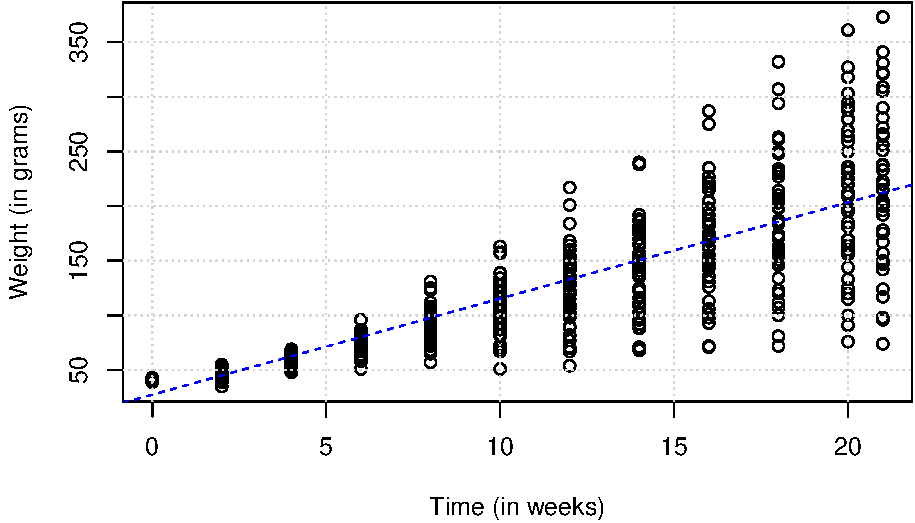
\includegraphics{finalpaper_example_files/figure-latex/unnamed-chunk-16-1.pdf}
\caption{\label{fig:unnamed-chunk-16}Scatterplot of chicken weights over
time.}
\end{figure}

A histogram of the weight data are presented in the next figure

\begin{Shaded}
\begin{Highlighting}[]
\CommentTok{# Task 9: Histogram}
\CommentTok{# INSERT CODE HERE}


\CommentTok{# Task 20: Custom Function: my.hist()}
\CommentTok{# Insert code here}
\end{Highlighting}
\end{Shaded}

\begin{figure}[htbp]
\centering
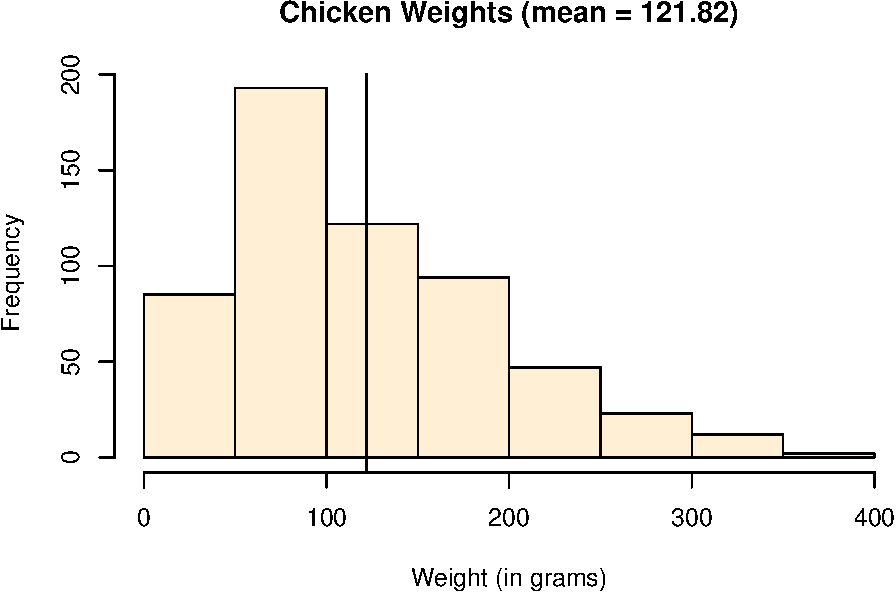
\includegraphics{finalpaper_example_files/figure-latex/unnamed-chunk-18-1.pdf}
\caption{\label{fig:unnamed-chunk-18}Distribution of weights across all data
points.}
\end{figure}

Histograms separately for each diet are displayed in the next figure

\begin{Shaded}
\begin{Highlighting}[]
\CommentTok{# Task 20: Loop}
\CommentTok{# INSERT CODE HERE}
\end{Highlighting}
\end{Shaded}

\begin{figure}[htbp]
\centering
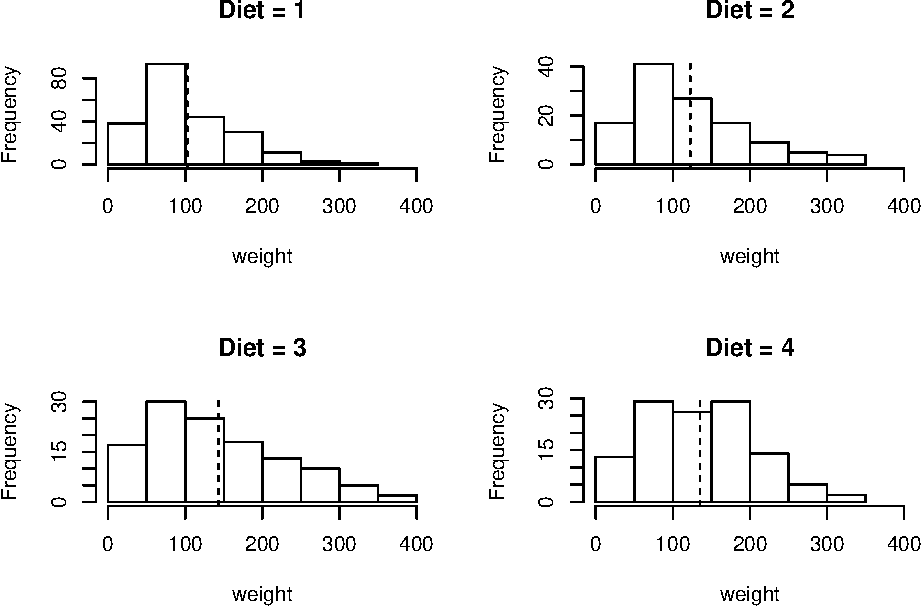
\includegraphics{finalpaper_example_files/figure-latex/unnamed-chunk-20-1.pdf}
\caption{\label{fig:unnamed-chunk-20}Histograms of the distribution of
weights across time for each diet. Vertical lines are means.}
\end{figure}

A pirateplot showing the relationship between diet and weight is shown
here:

\begin{Shaded}
\begin{Highlighting}[]
\CommentTok{# Task 10: pirateplot}
\CommentTok{# INSERT CODE HERE}
\end{Highlighting}
\end{Shaded}

\begin{figure}[htbp]
\centering
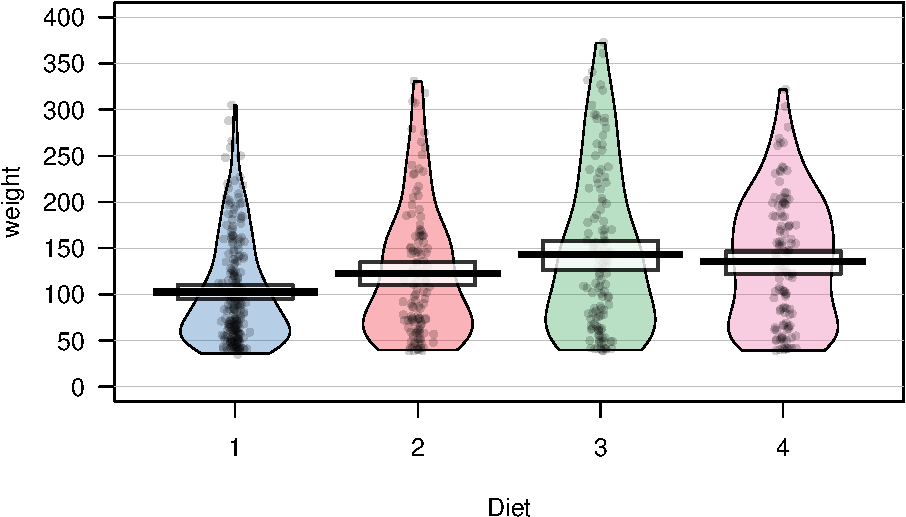
\includegraphics{finalpaper_example_files/figure-latex/unnamed-chunk-22-1.pdf}
\caption{\label{fig:unnamed-chunk-22}Pirateplot showing the distribution of
chicken weights by diet. Horizontal lines show means while white boxes
show Bayesian 95\% highest density intervals.}
\end{figure}

The mean weight of chicks on each diet is shown in the following table:

\begin{Shaded}
\begin{Highlighting}[]
\CommentTok{# Task 11: Descriptive statistics across groups}
\CommentTok{# INSERT CODE HERE}
\end{Highlighting}
\end{Shaded}

\begin{table}[tbp]
\begin{center}
\begin{threeparttable}
\caption{\label{tab:unnamed-chunk-24}Mean weights of chickens on each diet}
\begin{tabular}{ll}
\toprule
Diet & \multicolumn{1}{c}{Mean Weight}\\
\midrule
1.00 & 102.65\\
2.00 & 122.62\\
3.00 & 142.95\\
4.00 & 135.26\\
\bottomrule
\end{tabular}
\end{threeparttable}
\end{center}
\end{table}

\begin{Shaded}
\begin{Highlighting}[]
\CommentTok{# Task 12: 1 sample t-test}
\CommentTok{# INSERT CODE HERE}
\end{Highlighting}
\end{Shaded}

\begin{verbatim}
## 
##  One Sample t-test
## 
## data:  ChickWeight$weight
## t = 7.3805, df = 577, p-value = 5.529e-13
## alternative hypothesis: true mean is not equal to 100
## 95 percent confidence interval:
##  116.0121 127.6246
## sample estimates:
## mean of x 
##  121.8183
\end{verbatim}

A one sample t-test comparing the weights of chickens to a null
hypothesis of 100 was significant \(M = 121.82\), 95\% CI \([116.01\),
\(127.62]\), \(t(577) = 7.38\), \(p < .001\). The mean weight of
chickens was significantly larger than 100 grams.

\begin{Shaded}
\begin{Highlighting}[]
\CommentTok{# Task 13: t-test with subset}
\CommentTok{# INSERT CODE HERE}
\end{Highlighting}
\end{Shaded}

\begin{verbatim}
## 
##  Welch Two Sample t-test
## 
## data:  weight by Diet
## t = -2.6378, df = 201.38, p-value = 0.008995
## alternative hypothesis: true difference in means is not equal to 0
## 95 percent confidence interval:
##  -34.899942  -5.042482
## sample estimates:
## mean in group 1 mean in group 2 
##        102.6455        122.6167
\end{verbatim}

A two sample t-test comparing the weights of chickens between diets 1
and 2 was significant \(\Delta M = 19.97\), 95\% CI \([-34.90\),
\(-5.04]\), \(t(201.38) = -2.64\), \(p = .009\), the weights of chickens
was significantly higher in diet 2 compared to diet 1.

\begin{Shaded}
\begin{Highlighting}[]
\CommentTok{# Task 14: correlation test}
\CommentTok{# INSERT CODE HERE}
\end{Highlighting}
\end{Shaded}

\begin{verbatim}
## 
##  Pearson's product-moment correlation
## 
## data:  Time and weight
## t = 36.725, df = 576, p-value < 2.2e-16
## alternative hypothesis: true correlation is not equal to 0
## 95 percent confidence interval:
##  0.8109073 0.8599481
## sample estimates:
##       cor 
## 0.8371017
\end{verbatim}

A correlation test detecting a relationship between time and weight was
significant \(r = .84\), 95\% CI \([.81\), \(.86]\), \(t(576) = 36.73\),
\(p < .001\), as time increased, the weight of chickens increased.

\begin{Shaded}
\begin{Highlighting}[]
\CommentTok{# Task 15: correlation test with subset}
\CommentTok{# INSERT CODE HERE}
\end{Highlighting}
\end{Shaded}

\begin{verbatim}
## 
##  Pearson's product-moment correlation
## 
## data:  Time and weight
## t = 15.449, df = 118, p-value < 2.2e-16
## alternative hypothesis: true correlation is not equal to 0
## 95 percent confidence interval:
##  0.7485471 0.8697470
## sample estimates:
##       cor 
## 0.8180325
\end{verbatim}

A correlation test detecting a relationship between time and weight only
for chickens on diet 2 was significant \(r = .82\), 95\% CI \([.75\),
\(.87]\), \(t(118) = 15.45\), \(p < .001\), as time increased, the
weight of chickens on diet 2 increased.

\begin{Shaded}
\begin{Highlighting}[]
\CommentTok{# Task 16: Chi-Square test}
\CommentTok{# INSERT CODE HERE}
\end{Highlighting}
\end{Shaded}

\begin{verbatim}
## 
##  Chi-squared test for given probabilities
## 
## data:  table(ChickWeight$Diet)
## X-squared = 52.616, df = 3, p-value = 2.214e-11
\end{verbatim}

To see if there was a significant difference in the number of chickes on
each diet. I performed a chi-square test. The test was significant
\(\chi^2(3, n = 578) = 52.62\), \(p < .001\), indicating that chickens
were not equally distributed amongst the diets.

\begin{Shaded}
\begin{Highlighting}[]
\CommentTok{# Task 17: ONE-WAY ANOVA}
\CommentTok{# INSERT CODE HERE}
\end{Highlighting}
\end{Shaded}

\begin{verbatim}
## Call:
##    aov(formula = weight ~ factor(Diet), data = ChickWeight)
## 
## Terms:
##                 factor(Diet) Residuals
## Sum of Squares      155862.7 2758693.3
## Deg. of Freedom            3       574
## 
## Residual standard error: 69.32594
## Estimated effects may be unbalanced
\end{verbatim}

\begin{verbatim}
##               Df  Sum Sq Mean Sq F value   Pr(>F)    
## factor(Diet)   3  155863   51954   10.81 6.43e-07 ***
## Residuals    574 2758693    4806                     
## ---
## Signif. codes:  0 '***' 0.001 '**' 0.01 '*' 0.05 '.' 0.1 ' ' 1
\end{verbatim}

To see if there was a significant difference in weights between diets, I
performed a one-way ANOVA. The test was significant , indicating that
there was a significant difference between diets. Post-hoc tests showed
significant differences between Diets 1 and 3 (diff = 40.30, p
\textless{} .01), and Diets 1 and 4 (diff = 32.62, p \textless{} .01).

\begin{Shaded}
\begin{Highlighting}[]
\CommentTok{# Task 18: TWO-WAY ANOVA}
\CommentTok{# INSERT CODE HERE}
\end{Highlighting}
\end{Shaded}

\begin{verbatim}
## Call:
##    aov(formula = weight ~ factor(Diet) + factor(Time), data = ChickWeight)
## 
## Terms:
##                 factor(Diet) factor(Time) Residuals
## Sum of Squares      155862.7    2040908.0  717785.2
## Deg. of Freedom            3           11       563
## 
## Residual standard error: 35.70615
## Estimated effects may be unbalanced
\end{verbatim}

\begin{verbatim}
##               Df  Sum Sq Mean Sq F value Pr(>F)    
## factor(Diet)   3  155863   51954   40.75 <2e-16 ***
## factor(Time)  11 2040908  185537  145.53 <2e-16 ***
## Residuals    563  717785    1275                   
## ---
## Signif. codes:  0 '***' 0.001 '**' 0.01 '*' 0.05 '.' 0.1 ' ' 1
\end{verbatim}

To see if there was a significant difference in weights between diets
and time points, I performed a two-way ANOVA. The effect of both diet
\(F(3, 563) = 40.75\), \(\mathrm{MSE} = 1,274.93\), \(p < .001\),
\(\eta^2_G = .178\) and time \(F(11, 563) = 145.53\),
\(\mathrm{MSE} = 1,274.93\), \(p < .001\), \(\eta^2_G = .740\) were
significant. Post-hoc tests showed significant differences between all
Diets except for 4 and 3 (diff = -7.69, p = 0.34). There were
significant differences between almost all pairs of time periods.

\begin{Shaded}
\begin{Highlighting}[]
\CommentTok{# Task 19: REGRESSION}
\CommentTok{# INSERT CODE HERE}
\end{Highlighting}
\end{Shaded}

\begin{verbatim}
## 
## Call:
## lm(formula = weight ~ Time, data = ChickWeight)
## 
## Coefficients:
## (Intercept)         Time  
##      27.467        8.803
\end{verbatim}

\begin{verbatim}
## 
## Call:
## lm(formula = weight ~ Time, data = ChickWeight)
## 
## Residuals:
##      Min       1Q   Median       3Q      Max 
## -138.331  -14.536    0.926   13.533  160.669 
## 
## Coefficients:
##             Estimate Std. Error t value Pr(>|t|)    
## (Intercept)  27.4674     3.0365   9.046   <2e-16 ***
## Time          8.8030     0.2397  36.725   <2e-16 ***
## ---
## Signif. codes:  0 '***' 0.001 '**' 0.01 '*' 0.05 '.' 0.1 ' ' 1
## 
## Residual standard error: 38.91 on 576 degrees of freedom
## Multiple R-squared:  0.7007, Adjusted R-squared:  0.7002 
## F-statistic:  1349 on 1 and 576 DF,  p-value: < 2.2e-16
\end{verbatim}

To see if time was related to weight, I regressed weight on time.
Results showed a significant positive effect of time \(b = 8.80\), 95\%
CI \([8.33\), \(9.27]\), \(t(576) = 36.73\), \(p < .001\),
\(R^2 = .70\), \(F(1, 576) = 1,348.74\), \(p < .001\)

\section{Conclusion}\label{conclusion}

The two most important results were that chickens gain weight over time,
and Diet 3 lead to the highest weights while Diet 1 lead to the lowest
weights.

\newpage

\section{References}\label{references}

\setlength{\parindent}{-0.5in} \setlength{\leftskip}{0.5in}






\end{document}
